\subsection{CFD Simulation vs. Collected flight data \& \texttt{OpenRocket} simulation}
\label{subsec:cfd_vs_flight_data}

Finally, the results of the simulation are compared with the data collected during the rocket launch and the results of the simulation run in \texttt{OpenRocket}.

\subsubsection{Flight data}
\label{subsubsec:flight_data}

To collect data, we used a BMP280 barometer/thermometer sensor, which was placed inside the nose cone of the rocket and connected to an Arduino Nano board.
Because of poor quality SD writer module however, we weren't able to sampling at a high frequency and the number of collected data is limited (but still sufficient for our purpose).

In Table \ref{tab:flight_data} we report all the data collected during the rocket launch:

\begin{table}[H]
    \centering
    \begin{tabular}{|c|c|}
        \hline
        \textbf{Time [s]} & \textbf{Altitude [m]} \\
        \hline
        $494.130$         & $1443$                \\
        $495.233$         & $1443$                \\
        $496.334$         & $1444$                \\
        $497.437$         & $1554$                \\
        $498.540$         & $1678$                \\
        $500.745$         & $1809$                \\
        $501.848$         & $1847$                \\
        $502.953$         & $1903$                \\
        $504.055$         & $1931$                \\
        $505.161$         & $1958$                \\
        $506.263$         & $1973$                \\
        $507.364$         & $1979$                \\
        $508.468$         & $1976$                \\
        $509.570$         & $1965$                \\
        \hline
    \end{tabular}
    \caption{Data collected during the rocket launch.}
    \label{tab:flight_data}
\end{table}

In Figure \ref{fig:flight_data}, both the data of Table \ref{tab:flight_data} and their interpolation are shown.

\begin{figure}[H]
    \centering
    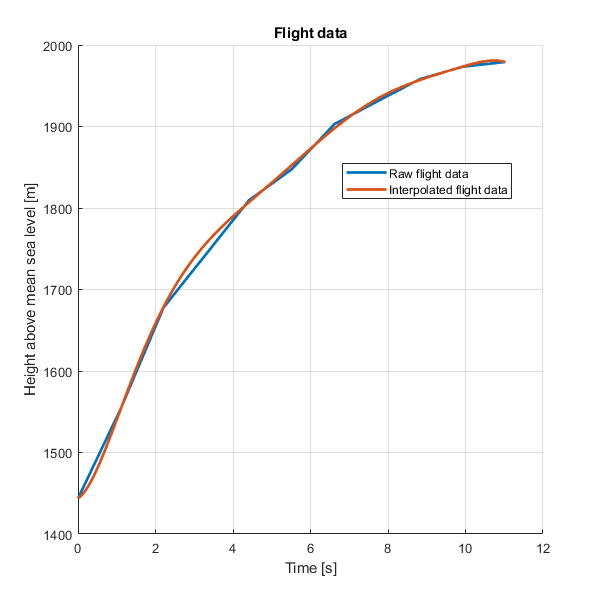
\includegraphics[width=.5\textwidth]{img/Validation/FlightData.png}
    \caption{Data collected during the rocket launch.}
    \label{fig:flight_data}
\end{figure}

For the interpolation, we used a Lagrange polynomial of degree $7$ (out of $10$ points) to obtain a smooth curve that can be used to compute also the vertical velocity of the rocket.


\subsubsection{\texttt{OpenRocket} simulation}
\label{subsubsec:openrocket_simulation}

As we have said, \texttt{OpenRocket} is a software that allows to both design and simulate the flight of a rocket.

By assigning shape, dimensions, mass, and an hypothetical $C_d$ to each component of the rocket, the software is able to give a raw estimation of the dynamics during the flight.
In Figure \ref{fig:openrocket_simulation}, the results of the simulation run in \texttt{OpenRocket} are shown.

\begin{figure}[H]
    \centering
    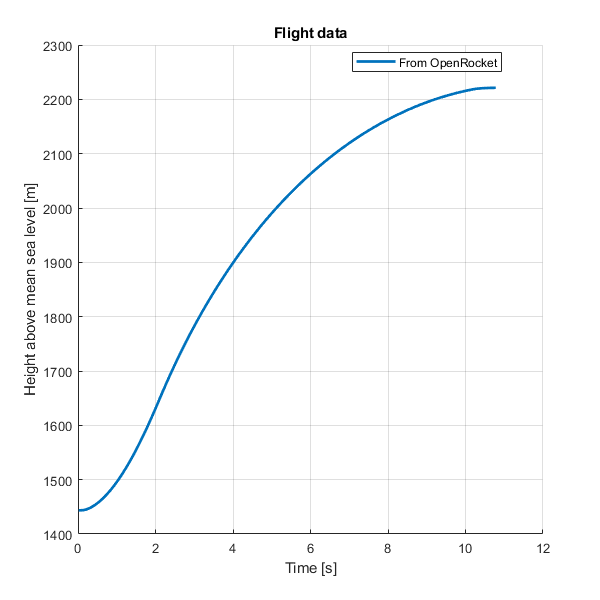
\includegraphics[width=.5\textwidth]{img/Validation/OpenRocket.png}
    \caption{Simulation run in \texttt{OpenRocket}.}
    \label{fig:openrocket_simulation}
\end{figure}


\subsubsection{Final comparison}
\label{subsubsec:final_comparison}

From Figure \ref{fig:flight_data} and Figure \ref{fig:openrocket_simulation}, we can see that the two curves (at the least in the apogee altitude) are not in agreement.

This is a common situation, as the simulation in \texttt{OpenRocket} are performed considering almost ideal condition and neglecting any possible aerodynamic imperfection of the rocket (which of course are present in the real world).

To overcome this discrepancy between the simulation and the real world, we will decrease the thrust curvature by a given factor until the peak velocity between the two curves are the same.
This might be a very strong assumption, but in reality in the world of model rocket is quite common as the effective thrust of the engine is almost always lower than the nominal thrust declared by the manufacturer.

Having said this, we can proceed with the comparison of the results of the CFD simulation with the collected flight data.

\paragraph{CFD simulation vs. \texttt{OpenRocket} simulation}

In Figure \ref{fig:comparison_flight_data}, the altitude and the vertical velocity of the rocket are shown.

\begin{figure}[H]
    \centering
    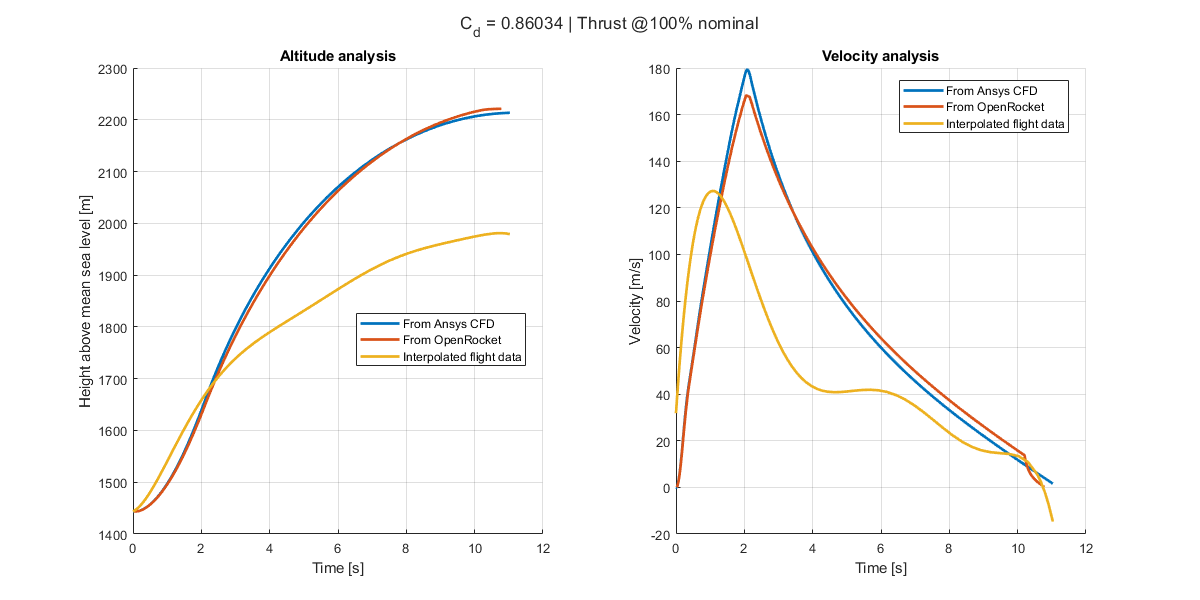
\includegraphics[width=\textwidth]{img/Validation/All_100.png}
    \caption{
        Comparison of the altitude and the vertical velocity of the rocket, considering a full thrust curve and $C_d = 0.86$ (from the CFD simulation).
        As the legend reports, the blue line represents the prediction based on the $C_d$ computed in the CFD simulation, the orange line represents the simulation run in \texttt{OpenRocket}, while the yellow line represents the collected flight data.
    }
    \label{fig:comparison_flight_data}
\end{figure}

As we can see, the curves generated with the CFD simulation and the one from \texttt{OpenRocket} are almost identical, while the collected flight data are way off.

\paragraph{CFD simulation vs. collected flight data}

However, as we have mentioned at the beginning of this section, the thrust curve of the engine are usually not accurate and often turns out to be much less than the nominal thrust declared by the manufacturer.
To overcome this discrepancy, we can decrease the thrust curve by a factor of $0.7$ until the peak velocity between the flight data and the CFD simulation are the same.
In this case, the results are shown in Figure \ref{fig:comparison_flight_data_70}.

\begin{figure}[H]
    \centering
    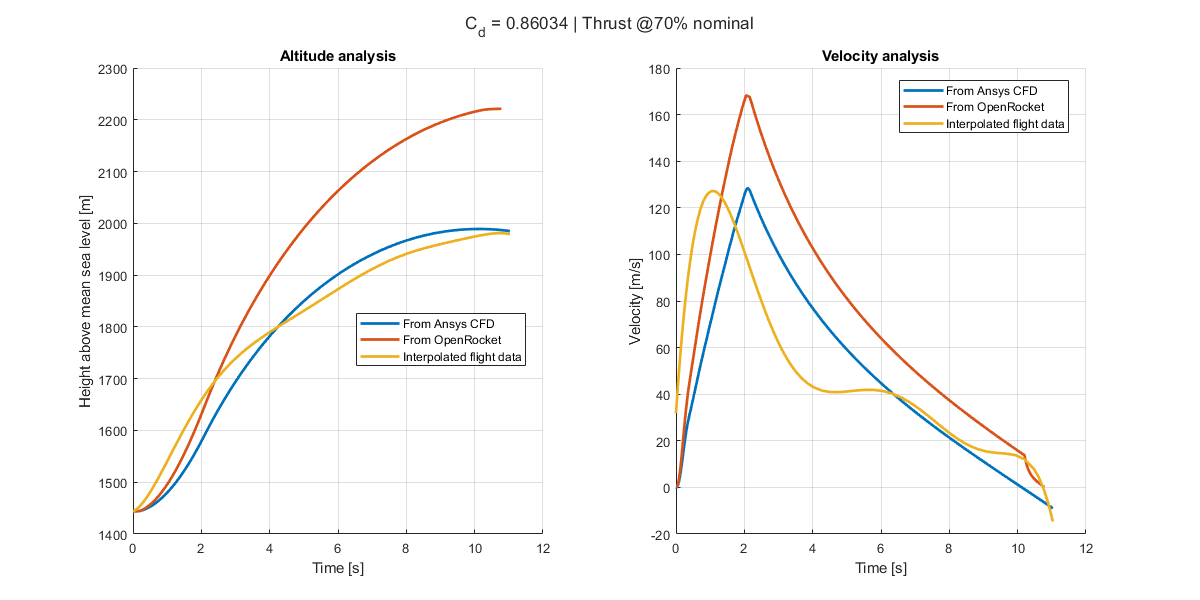
\includegraphics[width=\textwidth]{img/Validation/All_70.png}
    \caption{Comparison of the altitude and the vertical velocity of the rocket, considering a thrust curve decreased by a factor of $0.7$ and $C_d = 0.86$ (from the CFD simulation).}
    \label{fig:comparison_flight_data_70}
\end{figure}

By decreasing the thrust curve by a factor of $0.7$, the peak velocity of the flight data and the CFD simulation are almost the same.
Even if collected data are few and of poor quality (see the strong non-physical oscillation in the velocity curve), we can still try to relate the two curves.
By doing so, we can see that the CFD simulation is in good agreement with the collected data, while the simulation run in \texttt{OpenRocket} of course is not.

\paragraph{\texttt{OpenRocket} coefficient of drag estimation}

One may also ask what's the coefficient of drag used in the \texttt{OpenRocket} simulation.
Unfortunately, the software doesn't provide this information, but we can try to estimate it by comparing the altitude estimation for different values of $C_d$ around the value computed in the CFD simulation.
In Table \ref{tab:openrocket_cd}, we report three different values of $C_d$ and the corresponding peak altitude and velocity computed using our simple model and the comparison with the simulation from \texttt{OpenRocket}.

\begin{table}[H]
    \centering
    \begin{tabular}{|c|c|c|}
        \hline
        $C_d$               & \textbf{Altitude @ $t=10s$ [m]} & \textbf{Peak velocity [m/s]} \\
        \texttt{OpenRocket} & $2.2166e+03$                    & $168.2810$                   \\
        $0.903$             & $2.1900e+03$                    & $177.6557$                   \\
        $0.860$             & $2.2068e+03$                    & $179.3001$                   \\
        $0.817$             & $2.2271e+03$                    & $180.9773$                   \\
        \hline
    \end{tabular}
    \caption{Comparison of the peak altitude and velocity for different values of $C_d$.}
    \label{tab:openrocket_cd}
\end{table}

In Table \ref{tab:openrocket_cd}, we presented the results for $C_d = 0.903$, $C_d = 0.860$ and $C_d = 0.817$ (that are respectively $5\%$ and $5\%$ lower and higher than the value computed in the CFD simulation).
As we can observe, the peak velocity is almost the same for the three values of $C_d$, while the peak altitude is slightly different.
In particular, the best correspondence with the \texttt{OpenRocket} simulation is obtained for $C_d = 0.860$.
Also, from a shape point of view, the curve obtained with $C_d = 0.860$ is the one that best fits the \texttt{OpenRocket} simulation.
